% ============================================================
%  Hp3 manuscript -- Supplementary Information   (self-contained upload folder)
% ------------------------------------------------------------
%  This folder (manuscript/supplementary/) is the complete SI upload package:
%    supplementary.pdf            <- build product, upload this
%    SupplementalData.xlsx        <- Data S1 (copy of the source-data workbook)
%    si_table_orf.tex/.._sg.tex   <- auto-generated tables (make_si_tables.py)
%    si_fig_phrog/.._viptree_sg.png <- auto-generated figures (make_si_figures.R)
%  Regenerate tables/figures:
%      python3 make_si_tables.py        # Table S1, Table S4
%      Rscript  make_si_figures.R       # Figure S2, Figure S3
%  Build (self-contained; .latexmkrc here sets xelatex):
%      latexmk supplementary.tex
%  Figure S1 path reaches the gitignored Dropbox tree two levels up
%  (../../analyses/data/121-figs/).
% ============================================================
\documentclass[11pt,a4paper]{article}

% ---- engine / fonts (xelatex; Times New Roman, matching the main text) ----
\usepackage{iftex}
\ifPDFTeX
  \usepackage[T1]{fontenc}\usepackage[utf8]{inputenc}\usepackage{textcomp}
\else
  \usepackage{fontspec}
  \defaultfontfeatures{Scale=MatchLowercase}
  \setmainfont{Times New Roman}
\fi

\usepackage[a4paper,margin=1in]{geometry}
\IfFileExists{microtype.sty}{\usepackage{microtype}}{}
\usepackage{setspace}\onehalfspacing
\setlength{\parindent}{0pt}\setlength{\parskip}{6pt plus 2pt minus 1pt}

\usepackage{amsmath}
\usepackage{graphicx}
\usepackage{caption}
\usepackage{float}
\usepackage{longtable,booktabs,array,calc}
\usepackage{hyperref}\hypersetup{hidelinks}
\captionsetup{labelfont=bf,font=small}

% ---- supplementary figure/table numbering: S1, S2, ... ----
\renewcommand{\thefigure}{S\arabic{figure}}
\renewcommand{\thetable}{S\arabic{table}}

\title{\bfseries Supplementary Information\\[4pt]
\large A novel lytic \emph{Aeromonas} bacteriophage rescues
largemouth bass from lethal \emph{Aeromonas hydrophila} infection}
\date{}

\begin{document}
\maketitle

\noindent This file contains the supplementary figures, tables, and data
supporting the main text.

\medskip
\noindent\textbf{Contents}
\begin{itemize}\setlength{\itemsep}{0pt}
\item \textbf{Figure S1.} Protein-sharing network of Hp3 and reference viruses (vConTACT3).
\item \textbf{Figure S2.} Functional-category distribution of the 105 Hp3 ORFs (PHROG).
\item \textbf{Figure S3.} Whole-proteome similarity ($S_G$) of Hp3 to 5,632 reference viruses (ViPTree).
\item \textbf{Table S1.} Genome annotation of Hp3 (105 ORFs).
\item \textbf{Table S2.} Antibiotic-resistance and virulence-gene screening.
\item \textbf{Table S3.} Survival analysis statistics (\emph{in vivo} challenge).
\item \textbf{Table S4.} Closest reference viruses to Hp3 by whole-proteome similarity ($S_G$).
\item \textbf{Table S5.} Nucleotide-level intergenomic similarity (VIRIDIC).
\item \textbf{Data S1.} Source data for the \emph{in vitro} and \emph{in vivo} experiments (Excel).
\end{itemize}

\clearpage
% ============================================================
%  Figure S1 -- vConTACT3 protein-sharing network (cited in main text)
% ============================================================
\begin{figure}[H]
\centering
\includegraphics[width=\linewidth,keepaspectratio]{../../analyses/data/121-figs/vc3.png}
\caption{\textbf{Protein-sharing network of phage Hp3 and reference
prokaryotic viruses (vConTACT3).} Each node is a viral genome; nodes are
joined when they share at least one protein cluster, and only viruses
connected to Hp3 are shown. Hp3 (green) groups closely with
\emph{Aeromonas} phage HJ05 (linked by a red edge) and, more distantly,
with \emph{Rhizobium} phage vB\_RleS\_L338C, together forming the highly
distinct Hp3--HJ05 genus. This cluster is clearly separated from
established families, including its nearest neighbours in the
\emph{Peduoviridae} and \emph{Straboviridae}. Node colour denotes the
family-level assignment given in the legend; ``Other unclassified''
(grey) marks genomes that currently lack a family-level classification.
The network was computed with vConTACT3 against the NCBI viral RefSeq
database (v230) and visualized in Cytoscape.}
\label{fig-vc3-network}
\end{figure}

\clearpage
% ============================================================
%  Figure S2 -- PHROG functional-category distribution (make_si_figures.R)
% ============================================================
\begin{figure}[H]
\centering
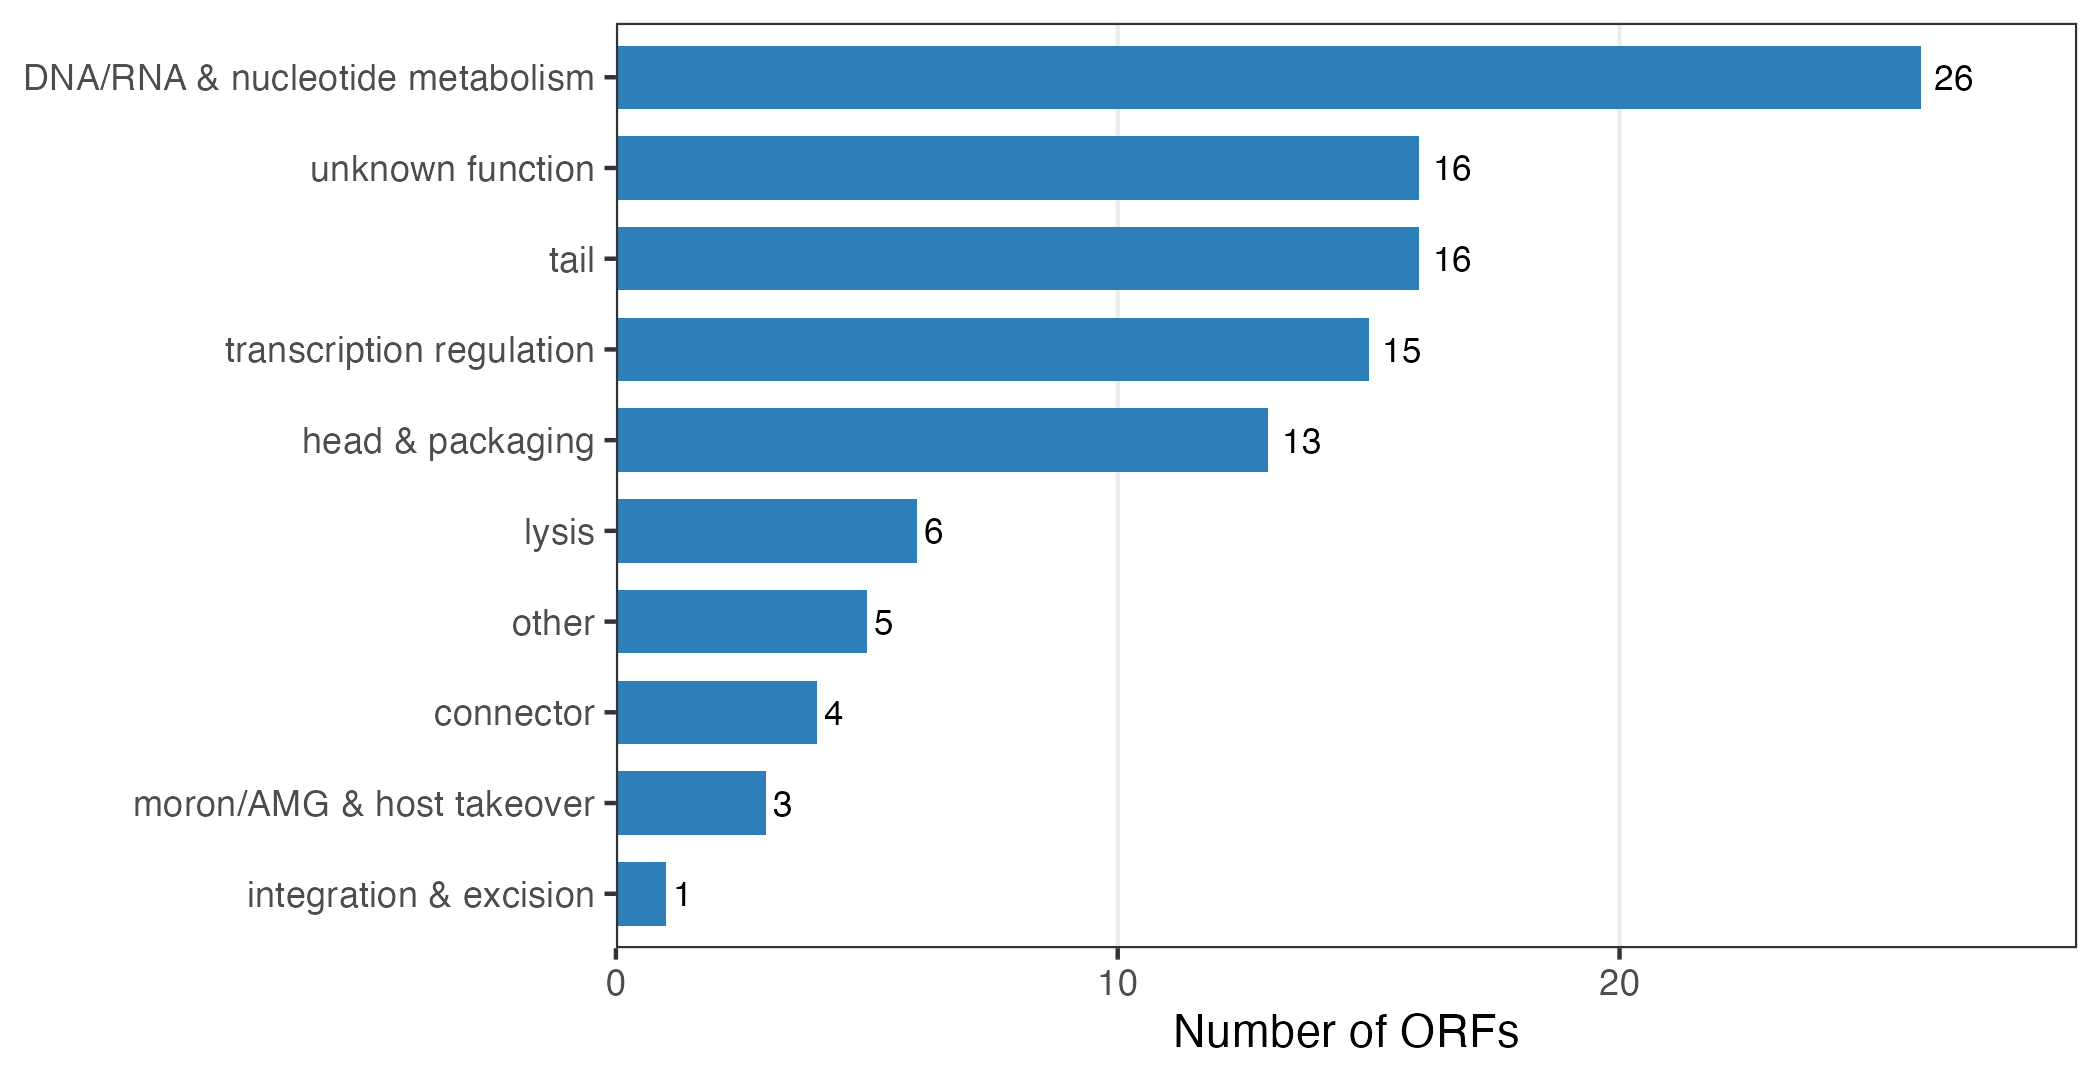
\includegraphics[width=0.92\linewidth,keepaspectratio]{si_fig_phrog.png}
\caption{\textbf{Functional-category distribution of the Hp3 genome.}
The 105 predicted ORFs (Table~S1) were grouped by PHROG functional category
after annotation with Pharokka, Phold, and Phynteny. Beyond the
structural modules typical of \emph{Caudoviricetes} (head and packaging,
connector, tail), the genome is notably enriched in DNA/RNA and
nucleotide-metabolism genes ($n=26$), consistent with a replication-
focused virulent lifestyle. A single ORF falls in the
integration-and-excision category (a transposase-like remnant; see
Table~S2 and main text), and no lysogeny-control module is present.}
\label{fig-phrog}
\end{figure}

\clearpage
% ============================================================
%  Figure S3 -- ViPTree S_G distribution (make_si_figures.R)
% ============================================================
\begin{figure}[H]
\centering
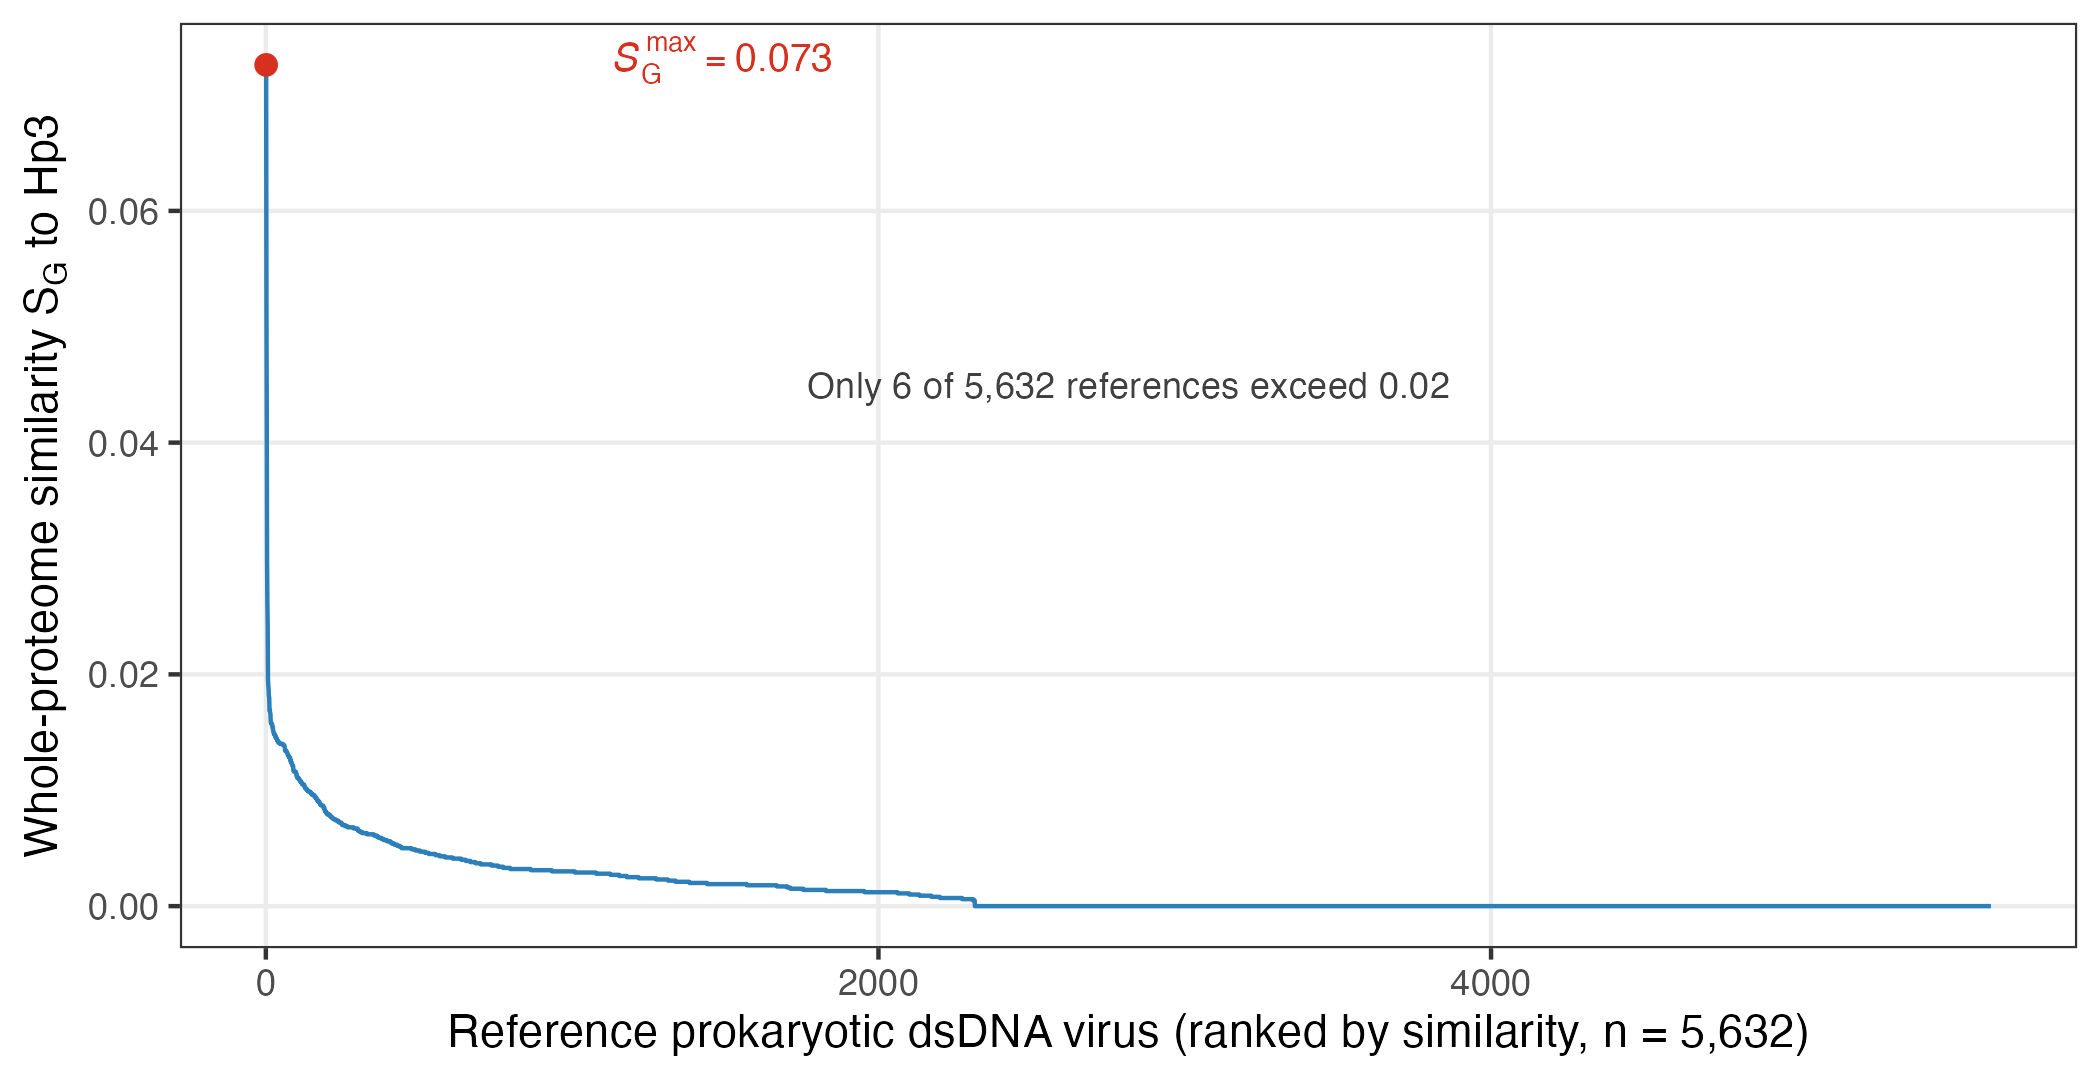
\includegraphics[width=0.92\linewidth,keepaspectratio]{si_fig_viptree_sg.png}
\caption{\textbf{Hp3 occupies an isolated region of viral sequence space.}
Whole-proteome genomic similarity ($S_G$, ViPTree) of Hp3 to each of the
5,632 reference prokaryotic dsDNA viruses, ranked in descending order. The
maximum $S_G$ is only 0.073 (red point; the unclassified \emph{Rhizobium}
phage vB\_RleS\_L338C), and only six references exceed $S_G=0.02$. The
rapid decay to near-zero similarity illustrates the deeply branching,
unclassified position of Hp3 reported in the main text and listed in
Table~S4.}
\label{fig-viptree-sg}
\end{figure}

\clearpage
% ============================================================
%  Table S1 -- full ORF annotation (auto-generated: make_si_tables.py)
% ============================================================
% AUTO-GENERATED by make_si_tables.py -- do not edit by hand.
\begin{small}
\begin{longtable}{@{}l l r p{0.22\linewidth} p{0.34\linewidth}@{}}
\caption{\textbf{Genome annotation of bacteriophage Hp3 (vB\_AhyM\_Hp3).} All 105 predicted open reading frames (ORFs) of the 84{,}750\,bp genome (GenBank PX754746.1), with genomic coordinates, length, PHROG functional category, and predicted product. Annotation combined Pharokka, Phold, and Phynteny.}\label{tbl-si-orf}\\
\toprule
\textbf{Locus tag} & \textbf{Position (bp)} & \textbf{Length} & \textbf{PHROG category} & \textbf{Predicted product}\\
\midrule
\endfirsthead
\toprule
\textbf{Locus tag} & \textbf{Position (bp)} & \textbf{Length} & \textbf{PHROG category} & \textbf{Predicted product}\\
\midrule
\endhead
\midrule \multicolumn{5}{r@{}}{\textit{continued on next page}}\\
\endfoot
\bottomrule
\endlastfoot
hp3\_0001 & 1--1,941 & 1,941 & head and packaging & terminase large subunit\\
hp3\_0002 & 1,880--3,040 & 1,161 & moron, auxiliary metabolic gene and host takeover & phospho-2-dehydro-3-deoxyheptonate aldolase\\
hp3\_0003 & 2,988--3,161 & 174 & unknown function & hypothetical protein\\
hp3\_0004 & 3,171--3,428 & 258 & unknown function & hypothetical protein\\
hp3\_0005 & 3,580--3,972 & 393 & unknown function & hypothetical protein\\
hp3\_0006 & 4,013--4,324 & 312 & transcription regulation & hypothetical protein\\
hp3\_0007 & 4,321--4,878 & 558 & transcription regulation & hypothetical protein\\
hp3\_0008 & 4,888--5,133 & 246 & transcription regulation & hypothetical protein\\
hp3\_0009 & 5,130--5,369 & 240 & transcription regulation & hypothetical protein\\
hp3\_0010 & 5,366--5,875 & 510 & transcription regulation & hypothetical protein\\
hp3\_0011 & 5,885--6,544 & 660 & transcription regulation & hypothetical protein\\
hp3\_0012 & 6,675--7,214 & 540 & transcription regulation & hypothetical protein\\
hp3\_0013 & 7,211--7,738 & 528 & transcription regulation & hypothetical protein\\
hp3\_0014 & 7,731--8,324 & 594 & unknown function & hypothetical protein\\
hp3\_0015 & 8,324--8,500 & 177 & DNA, RNA and nucleotide metabolism & hypothetical protein\\
hp3\_0016 & 8,497--8,832 & 336 & DNA, RNA and nucleotide metabolism & hypothetical protein\\
hp3\_0017 & 8,832--9,416 & 585 & DNA, RNA and nucleotide metabolism & hypothetical protein\\
hp3\_0018 & 9,488--10,477 & 990 & DNA, RNA and nucleotide metabolism & dATP / dGTP pyrophosphohydrolase\\
hp3\_0019 & 10,562--11,359 & 798 & DNA, RNA and nucleotide metabolism & hypothetical protein\\
hp3\_0020 & 11,437--11,892 & 456 & moron, auxiliary metabolic gene and host takeover & membrane protein\\
hp3\_0021 & 11,892--12,338 & 447 & unknown function & hypothetical protein\\
hp3\_0022 & 12,335--13,552 & 1,218 & moron, auxiliary metabolic gene and host takeover & VFDB virulence factor protein\\
hp3\_0023 & 13,630--14,688 & 1,059 & transcription regulation & hypothetical protein\\
hp3\_0024 & 14,693--15,172 & 480 & transcription regulation & hypothetical protein\\
hp3\_0025 & 15,289--15,609 & 321 & transcription regulation & Arc-like repressor\\
hp3\_0026 & 15,672--16,349 & 678 & transcription regulation & hypothetical protein\\
hp3\_0027 & 16,435--16,752 & 318 & transcription regulation & hypothetical protein\\
hp3\_0028 & 16,792--17,355 & 564 & unknown function & hypothetical protein\\
hp3\_0029 & 17,352--18,197 & 846 & other & methyltransferase\\
hp3\_0030 & 18,300--18,602 & 303 & unknown function & hypothetical protein\\
hp3\_0031 & 18,602--18,919 & 318 & unknown function & hypothetical protein\\
hp3\_0032 & 18,916--19,242 & 327 & DNA, RNA and nucleotide metabolism & hypothetical protein\\
hp3\_0033 & 19,287--19,703 & 417 & DNA, RNA and nucleotide metabolism & hypothetical protein\\
hp3\_0034 & 19,703--20,209 & 507 & DNA, RNA and nucleotide metabolism & hypothetical protein\\
hp3\_0035 & 20,316--21,521 & 1,206 & DNA, RNA and nucleotide metabolism & Rnase H\\
hp3\_0036 & 21,463--22,425 & 963 & DNA, RNA and nucleotide metabolism & thymidylate synthase\\
hp3\_0037 & 22,546--24,291 & 1,746 & head and packaging & portal protein\\
hp3\_0038 & 24,254--25,198 & 945 & head and packaging & head morphogenesis\\
hp3\_0039 & 25,213--25,812 & 600 & other & protease\\
hp3\_0040 & 25,870--27,207 & 1,338 & head and packaging & head maturation protease\\
hp3\_0041 & 27,260--28,186 & 927 & head and packaging & virion structural protein\\
hp3\_0042 & 28,223--28,576 & 354 & head and packaging & hypothetical protein\\
hp3\_0043 & 28,533--28,754 & 222 & head and packaging & hypothetical protein\\
hp3\_0044 & 28,769--29,395 & 627 & connector & head-tail adaptor\\
hp3\_0045 & 29,392--29,853 & 462 & connector & head closure Hc1\\
hp3\_0046 & 29,863--30,303 & 441 & connector & tail completion or Neck1 protein\\
hp3\_0047 & 30,300--30,992 & 693 & head and packaging & portal protein\\
hp3\_0048 & 30,976--32,133 & 1,158 & tail & baseplate spike\\
hp3\_0049 & 32,143--32,871 & 729 & tail & hypothetical protein\\
hp3\_0050 & 32,883--33,248 & 366 & tail & baseplate wedge subunit\\
hp3\_0051 & 33,245--34,150 & 906 & tail & baseplate protein\\
hp3\_0052 & 34,154--35,410 & 1,257 & tail & tail protein\\
hp3\_0053 & 35,394--35,879 & 486 & head and packaging & virion structural protein\\
hp3\_0054 & 35,895--37,814 & 1,920 & tail & baseplate wedge subunit\\
hp3\_0055 & 37,828--39,045 & 1,218 & tail & tail fiber protein\\
hp3\_0056 & 39,057--39,278 & 222 & tail & hypothetical protein\\
hp3\_0057 & 39,327--40,982 & 1,656 & tail & minor tail protein\\
hp3\_0058 & 40,995--41,918 & 924 & DNA, RNA and nucleotide metabolism & anaerobic ribonucleoside reductase large subunit\\
hp3\_0059 & 41,938--42,504 & 567 & tail & hypothetical protein\\
hp3\_0060 & 42,620--44,224 & 1,605 & tail & tail sheath\\
hp3\_0061 & 44,261--44,767 & 507 & connector & head closure\\
hp3\_0062 & 44,827--45,153 & 327 & tail & tail protein\\
hp3\_0063 & 45,376--48,000 & 2,625 & tail & tail length tape measure protein\\
hp3\_0064 & 48,000--48,419 & 420 & tail & tail protein\\
hp3\_0065 & 48,419--48,658 & 240 & tail & baseplate hub\\
hp3\_0066 & 48,660--49,679 & 1,020 & tail & tail protein\\
hp3\_0067 & 49,690--50,004 & 315 & head and packaging & hypothetical protein\\
hp3\_0068 & 50,063--50,374 & 312 & lysis & hypothetical protein\\
hp3\_0069 & 50,393--50,830 & 438 & lysis & holin\\
hp3\_0070 & 50,837--51,520 & 684 & lysis & amidase\\
hp3\_0071 & 51,520--51,903 & 384 & unknown function & hypothetical protein\\
hp3\_0072 & 51,909--52,157 & 249 & unknown function & hypothetical protein\\
hp3\_0073 & 52,489--54,159 & 1,671 & other & ATPase\\
hp3\_0074 & 54,288--54,914 & 627 & unknown function & hypothetical protein\\
hp3\_0075 & 54,967--55,392 & 426 & DNA, RNA and nucleotide metabolism & hypothetical protein\\
hp3\_0076 & 55,392--55,595 & 204 & unknown function & hypothetical protein\\
hp3\_0077 & 55,606--55,977 & 372 & DNA, RNA and nucleotide metabolism & hypothetical protein\\
hp3\_0078 & 56,080--57,468 & 1,389 & DNA, RNA and nucleotide metabolism & replication initiation O-like\\
hp3\_0079 & 57,470--58,339 & 870 & DNA, RNA and nucleotide metabolism & hypothetical protein\\
hp3\_0080 & 58,343--58,924 & 582 & unknown function & hypothetical protein\\
hp3\_0081 & 58,921--60,342 & 1,422 & DNA, RNA and nucleotide metabolism & DnaB-like replicative helicase\\
hp3\_0082 & 60,371--63,100 & 2,730 & DNA, RNA and nucleotide metabolism & DNA polymerase\\
hp3\_0083 & 63,259--63,804 & 546 & unknown function & hypothetical protein\\
hp3\_0084 & 63,835--64,416 & 582 & DNA, RNA and nucleotide metabolism & hypothetical protein\\
hp3\_0085 & 64,418--65,452 & 1,035 & DNA, RNA and nucleotide metabolism & DNA primase\\
hp3\_0086 & 65,495--65,827 & 333 & unknown function & hypothetical protein\\
hp3\_0087 & 65,833--66,909 & 1,077 & DNA, RNA and nucleotide metabolism & single strand DNA binding protein\\
hp3\_0088 & 66,925--68,355 & 1,431 & DNA, RNA and nucleotide metabolism & DNA helicase\\
hp3\_0089 & 68,324--68,845 & 522 & transcription regulation & transcriptional regulator\\
hp3\_0090 & 68,946--69,194 & 249 & unknown function & hypothetical protein\\
hp3\_0091 & 69,194--70,438 & 1,245 & other & UvsX-like recombinase\\
hp3\_0092 & 70,443--70,808 & 366 & DNA, RNA and nucleotide metabolism & Holliday junction resolvase\\
hp3\_0093 & 70,810--71,874 & 1,065 & DNA, RNA and nucleotide metabolism & exonuclease\\
hp3\_0094 & 71,874--72,488 & 615 & DNA, RNA and nucleotide metabolism & RuvC-like Holliday junction resolvase\\
hp3\_0095 & 72,610--74,424 & 1,815 & head and packaging & head morphogenesis\\
hp3\_0096 & 74,529--77,267 & 2,739 & head and packaging & virion structural protein\\
hp3\_0097 & 77,310--77,549 & 240 & head and packaging & hypothetical protein\\
hp3\_0098 & 77,542--78,516 & 975 & lysis & hypothetical protein\\
hp3\_0099 & 78,661--78,921 & 261 & lysis & holin\\
hp3\_0100 & 78,961--79,278 & 318 & lysis & hypothetical protein\\
hp3\_0101 & 79,297--79,806 & 510 & transcription regulation & hypothetical protein\\
hp3\_0102 & 80,477--81,361 & 885 & DNA, RNA and nucleotide metabolism & ParB-like partition protein\\
hp3\_0103 & 81,409--83,001 & 1,593 & DNA, RNA and nucleotide metabolism & ParB-like partition nuclease\\
hp3\_0104 & 83,024--83,761 & 738 & other & tRNA methyltransferase\\
hp3\_0105 & 83,768--84,739 & 972 & integration and excision & transposase\\
\end{longtable}
\end{small}


\clearpage
% ============================================================
%  Table S2 -- resistance / virulence screen
% ============================================================
\begin{table}[H]\centering
\caption{\textbf{Antibiotic-resistance and virulence-gene screening of the
Hp3 genome.} Sequence-homology screens (Pharokka) against CARD and VFDB
returned no hits. The only flags arose from remote \emph{structural}
homology (Phold/Foldseek) at low identity and without any corresponding
sequence-homology hit, and are therefore not interpreted as functional
determinants (see main text).}\label{tbl-si-safety}
\begin{small}
\begin{tabular}{@{}l l l l@{}}
\toprule
\textbf{Screen} & \textbf{Method} & \textbf{Database} & \textbf{Result}\\
\midrule
Antibiotic resistance & Sequence homology (Pharokka) & CARD & No hits \\
Virulence (sequence)  & Sequence homology (Pharokka) & VFDB & No hits \\
Virulence (structure) & Structural homology (Phold/Foldseek) & VFDB & hp3\_0022 vs VFG047113, \\
 & & & \quad fident $=0.16$; no sequence hit \\
Integrase / mobility  & Structural homology (Phold/Foldseek) & --- & hp3\_0105 transposase-like, \\
 & & & \quad structural id.\ $=0.24$; no sequence hit \\
Lifestyle             & BACPHLIP & --- & Virulent ($P_{\mathrm{lytic}}=0.97$) \\
\bottomrule
\end{tabular}
\end{small}
\end{table}

% ============================================================
%  Table S3 -- survival statistics
% ============================================================
\begin{table}[H]\centering
\caption{\textbf{Survival analysis for the largemouth bass challenge
(Figure 5B).} Seven-day survival per group, pairwise Log-rank
(Mantel--Cox) tests with Benjamini--Hochberg adjustment, and a Cox
proportional-hazards estimate of the treatment effect. The PBS and
phage-only groups recorded no deaths and were excluded from the Cox
model.}\label{tbl-si-survival}
\begin{small}
\begin{tabular}{@{}l l@{}}
\toprule
\multicolumn{2}{@{}l}{\textit{Seven-day survival (n = 20 per group)}}\\
PBS control & 100\% \\
Phage-only & 100\% \\
\emph{A. hydrophila} (bacterial) & 15\% \\
Treatment (\emph{A. hydrophila} + Hp3, MOI 1.0) & 85\% \\
\midrule
\multicolumn{2}{@{}l}{\textit{Overall Log-rank test}}\\
$k$-sample (4 groups) & $\chi^2 = 64.6$, df $= 3$, $p = 6.2\times10^{-14}$ \\
\midrule
\multicolumn{2}{@{}l}{\textit{Pairwise Log-rank (Benjamini--Hochberg-adjusted)}}\\
Treatment vs.\ bacterial & $\chi^2 = 20.474$, $p_{\mathrm{adj}} = 1.2\times10^{-5}$ \\
Treatment vs.\ PBS & $p_{\mathrm{adj}} = 0.09$ \\
Treatment vs.\ phage-only & $p_{\mathrm{adj}} = 0.09$ \\
\midrule
\multicolumn{2}{@{}l}{\textit{Cox proportional-hazards (bacterial = reference)}}\\
Treatment hazard ratio & HR $= 0.091$, 95\% CI $0.026$--$0.320$, $p = 1.8\times10^{-4}$ \\
\bottomrule
\end{tabular}
\end{small}
\end{table}

\clearpage
% ============================================================
%  Table S4 -- ViPTree S_G top hits (auto-generated: make_si_tables.py)
% ============================================================
% AUTO-GENERATED by make_si_tables.py -- do not edit by hand.
\begin{table}[H]\centering
\caption{\textbf{Whole-proteome genomic similarity ($S_G$) of the closest reference prokaryotic viruses to Hp3 (ViPTree).} The maximum $S_G$ to any of the 5{,}633 reference dsDNA viruses is only 0.073, to the unclassified \emph{Rhizobium} phage vB\_RleS\_L338C, underscoring the isolated, deeply branching position of Hp3 reported in the main text.}\label{tbl-si-sg}
\begin{small}
\begin{tabular}{@{}r l l r@{}}
\toprule
\textbf{Rank} & \textbf{Reference virus} & \textbf{Family / host group} & \textbf{$S_G$ to Hp3}\\
\midrule
1 & Rhizobium phage vB\_RleS\_L338C & Pseudomonadota & 0.073\\
2 & Pseudomonas phage SM1 & Pseudomonadota & 0.052\\
3 & Acidithiobacillus phage AcaML1 & Pseudomonadota & 0.042\\
4 & Stenotrophomonas phage vB\_SmaS\_DLP\_5 & Pseudomonadota & 0.030\\
5 & Vibrio phage SIO-2 & Pseudomonadota & 0.026\\
6 & Vibrio phage 1 & Pseudomonadota & 0.024\\
7 & Achromobacter phage Mano & Pseudomonadota & 0.019\\
8 & Streptomyces phage Gilgamesh & Actinomycetota & 0.019\\
9 & Burkholderia phage Mica & Pseudomonadota & 0.019\\
10 & Streptomyces phage TurkishDelight & Actinomycetota & 0.018\\
11 & Pseudomonas phage Persinger & Pseudomonadota & 0.018\\
12 & Vibrio phage vB\_VpaM\_MAR & Pseudomonadota & 0.017\\
\bottomrule
\end{tabular}
\end{small}
\end{table}


% ============================================================
%  Table S5 -- VIRIDIC nucleotide-level intergenomic similarity
% ============================================================
\begin{table}[H]\centering
\caption{\textbf{Nucleotide-level intergenomic similarity (VIRIDIC).}
Pairwise intergenomic similarity among Hp3, its closest relative
\emph{Aeromonas} phage HJ05, and the protein-network-linked \emph{Rhizobium}
phage vB\_RleS\_L338C. Hp3 and HJ05 fall within one genus (VIRIDIC genus
threshold $\geq$70\%, species threshold $\geq$95\%), whereas the
vConTACT3 protein-sharing link to L338C corresponds to negligible
nucleotide identity.}\label{tbl-si-viridic}
\begin{small}
\begin{tabular}{@{}l r p{0.42\linewidth}@{}}
\toprule
\textbf{Genome pair} & \textbf{Similarity (\%)} & \textbf{Interpretation}\\
\midrule
Hp3 vs.\ HJ05 (OQ594355) & 83.65 & Same genus ($\geq$70\%), different species ($<$95\%) \\
Hp3 vs.\ vB\_RleS\_L338C (NC\_023502) & 3.00 & Unrelated at nucleotide level (vConTACT3 artifact) \\
HJ05 vs.\ vB\_RleS\_L338C & 3.22 & Unrelated at nucleotide level \\
\bottomrule
\end{tabular}
\end{small}
\end{table}

% ============================================================
%  Data S1 -- source-data workbook
% ============================================================
\bigskip
\noindent\textbf{Data S1. Source data for the \emph{in vitro} and
\emph{in vivo} experiments.} An Excel workbook (\texttt{SupplementalData.xlsx},
provided as a separate file in this folder) containing the raw measurements
underlying the one-step growth curve, thermal- and pH-stability assays,
optimal-MOI determination, 48-h lysis curves, and the seven-day survival
experiment. Figure source data are additionally archived in Figshare
(\href{https://doi.org/10.6084/m9.figshare.30500525}{10.6084/m9.figshare.30500525}).

\end{document}
